%
% tikztemplate.tex -- template for standalon tikz images
%
% (c) 2019 Prof Dr Andreas Müller, Hochschule Rapperswil
%

\documentclass[tikz]{standalone}
\usepackage{amsmath}
\usepackage{times}
\usepackage{txfonts}
\usepackage{pgfplots}
\usepackage{csvsimple}
\usetikzlibrary{arrows,intersections,math}
\begin{document}
	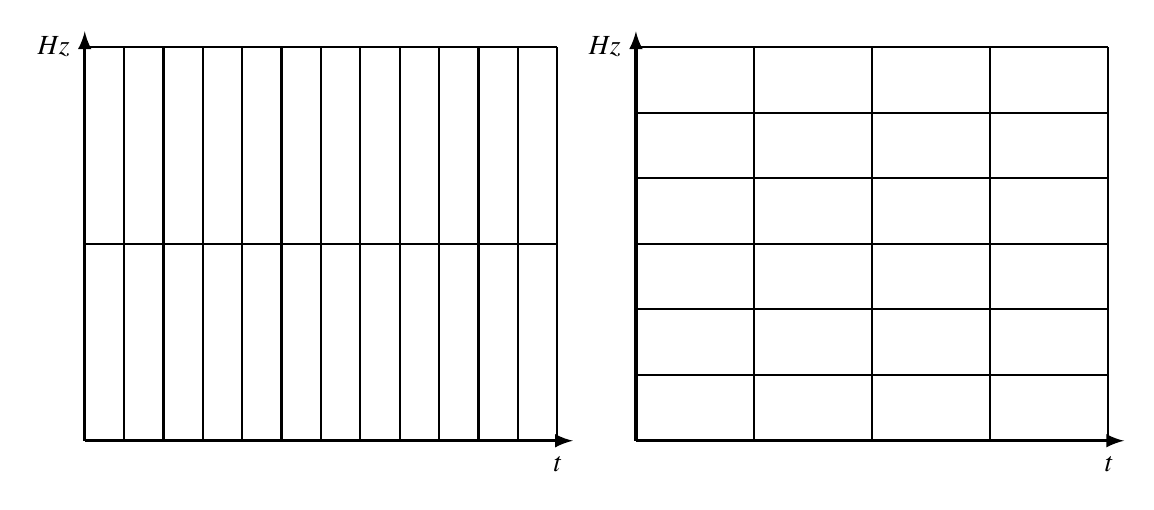
\begin{tikzpicture}[>=latex]
	\draw (6,-5.3) node{$t$};
	\draw (-0.4,0) node{$Hz$};
	\draw[->, very thick] (0,-5)--(0,0.2);
	\draw[->, very thick] (0,-5)--(6.2,-5);
	
	\draw[thick] (0,-0)--(6,-0);
	\draw[thick] (0,-2.5)--(6,-2.5);
	
	\draw[thick] (0.5,-5)--(0.5,0);
	\draw[thick] (1,-5)--(1,0);
	\draw[thick] (1.5,-5)--(1.5,0);
	\draw[thick] (2,-5)--(2,0);
	\draw[thick] (2.5,-5)--(2.5,0);
	\draw[thick] (3,-5)--(3,0);
	\draw[thick] (3.5,-5)--(3.5,0);
	\draw[thick] (4,-5)--(4,0);
	\draw[thick] (4.5,-5)--(4.5,0);
	\draw[thick] (5,-5)--(5,0);
	\draw[thick] (5.5,-5)--(5.5,0);
	\draw[thick] (6,-5)--(6,0);
	
	\draw (13,-5.3) node{$t$};
	\draw (6.6,0) node{$Hz$};
	\draw[->, very thick] (7,-5)--(7,0.2);
	\draw[->, very thick] (7,-5)--(13.2,-5);
	
	\draw[thick] (7,-0)--(13,-0);
	\draw[thick] (7,-0.833)--(13,-0.833);
	\draw[thick] (7,-1.666)--(13,-1.666);
	\draw[thick] (7,-2.499)--(13,-2.499);
	\draw[thick] (7,-3.33)--(13,-3.33);
	\draw[thick] (7,-4.166)--(13,-4.166);
	
	\draw[thick] (8.5,-5)--(8.5,0);
	\draw[thick] (10,-5)--(10,0);
	\draw[thick] (11.5,-5)--(11.5,0);
	\draw[thick] (13,-5)--(13,0);
	
	\end{tikzpicture}
\end{document}
